\section{Implementazione Algoritmo}
Nel capitolo precedente si è descritta la fase di sviluppo dell'algoritmo, ed il relativo pseudocodice.
Nel corso dell'iterazione 3 l'algoritmo è stato implementato in Spring. In particolare, la sua implementazione è strettamente legata
all'introduzione di nuove API quali quella per la selezione dei partecipanti e la gestione del profilo dell'utente.
Innanzitutto, per l' algoritmo è stato aggiunto un metodo nell'interfaccia EventsManagementIF responsabile della chiamata all'implementazione
effettiva dell'algoritmo, spezzata in due metodi separati (privati) per garantire una maggiore leggibilità. Il nuovo metodo
in EventService consente, oltre che di chiamare l'algoritmo, anche di aggiornare se ogni singola prenotazione per quell'evento 
è confermata o meno, andando ad aggiornare il campo "confirmation".
Successivamente, si è introdotto il calcolo del livello del profilo dell'utente, che viene eseguito considerando la media delle difficoltà
associate a ciascun evento al quale l'utente ha preso effettivamente parte.
\newpage
\subsection{UML sequence diagram}
E' possibile visualizzare le interazioni tra i metodi sviluppati per l'implementazione dell'algoritmo tramite un UML Sequence diagram.
\begin{center}
\begin{figure}[h!]
    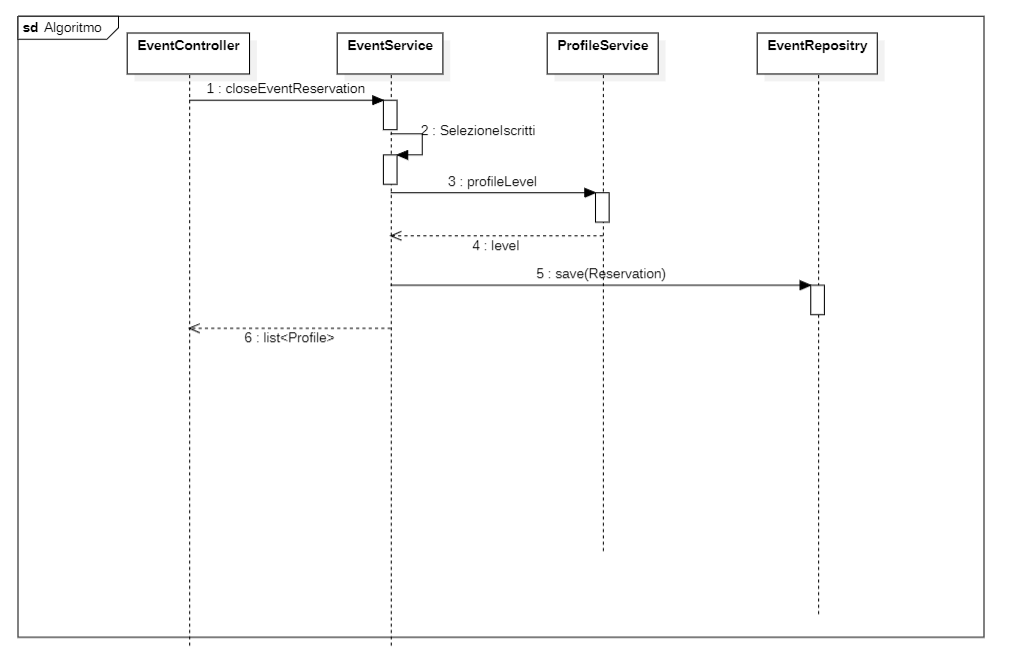
\includegraphics[width=1\textwidth]{Iterazione 3/images/sequence_diagram.png}
    \caption{Sequence diagram}\label{fig:seq}
  \end{figure}
\end{center}
